\begin{figure}[!ht]
    \centering
    \vspace{0.5cm}
    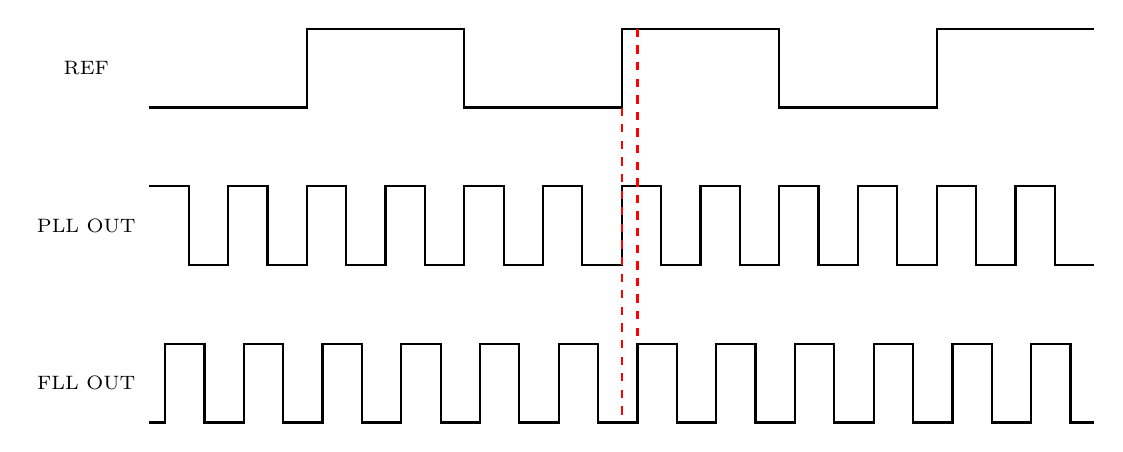
\begin{tikzpicture}

    \def \lref {0}
    \def \href {1}
    \def \loutpll {-2}
    \def \houtpll {-1}
    \def \loutfll {-4}
    \def \houtfll {-3}

    % Top signal: 3 periods of 4ns
    \draw[thick] (0,\lref) -- (2,\lref) -- (2,\href) -- (4,\href) -- (4,\lref) -- (6,\lref) -- (6,\href) -- (8,\href) -- (8,\lref) -- (10,\lref) -- (10,\href) -- (12,\href);
    %\draw[thick] (0,\href) -- (0.2,\href) -- (0.2,\lref) -- (2.2,\lref) -- (2.2,\href) -- (4.2,\href) -- (4.2,\lref) -- (6.2,\lref) -- (6.2,\href) -- (8.2,\href) -- (8.2,\lref) -- (10.2,\lref) -- (10.2,\href) -- (12,\href);
    \node at (-0.8,0.5) {\scriptsize REF};

    %\draw (2,-0.45) node[anchor=north]{\scriptsize $T_\text{REF}$};
    %\draw[<->] (0,-0.4) -- (4,-0.4);
    
    % Bottom signal: 12 periods of 1ns
    \draw[thick] (0,\houtpll) -- (0.5,\houtpll) -- (0.5,\loutpll) -- (1,\loutpll) -- (1,\houtpll) -- (1.5,\houtpll) -- (1.5,\loutpll) -- (2,\loutpll) -- (2,\houtpll) -- (2.5, \houtpll) -- (2.5,\loutpll) -- (3,\loutpll) -- (3,\houtpll) -- (3.5,\houtpll) -- (3.5,\loutpll) -- (4,\loutpll) -- (4,\houtpll) -- (4.5,\houtpll) -- (4.5,\loutpll) -- (5,\loutpll) -- (5,\houtpll) -- (5.5,\houtpll) -- (5.5,\loutpll) -- (6,\loutpll) -- (6,\houtpll) -- (6.5,\houtpll) -- (6.5,\loutpll) -- (7,\loutpll) -- (7,\houtpll) -- (7.5,\houtpll) -- (7.5,\loutpll) -- (8,\loutpll) -- (8,\houtpll) -- (8.5,\houtpll) -- (8.5,\loutpll) -- (9,\loutpll) -- (9,\houtpll) -- (9.5,\houtpll) -- (9.5,\loutpll) -- (10,\loutpll) -- (10,\houtpll) -- (10.5,\houtpll) -- (10.5,\loutpll) -- (11,\loutpll) -- (11,\houtpll) -- (11.5,\houtpll) -- (11.5,\loutpll) -- (12,\loutpll);
    \node at (-0.8,-1.5) {\scriptsize PLL OUT};

    %\draw (0.5,-2.95) node[anchor=north]{\scriptsize $T_\text{OUT\_PLL}$};
    %\draw[<->] (0,-2.9) -- (1,-2.9);
    
    \draw[thick] (0,\loutfll) -- (0.2,\loutfll) -- (0.2,\houtfll) -- (0.7,\houtfll) -- (0.7,\loutfll) -- (1.2,\loutfll) -- (1.2,\houtfll) -- (1.7,\houtfll) -- (1.7,\loutfll) -- (2.2,\loutfll) -- (2.2,\houtfll) -- (2.7, \houtfll) -- (2.7,\loutfll) -- (3.2,\loutfll) -- (3.2,\houtfll) -- (3.7,\houtfll) -- (3.7,\loutfll) -- (4.2,\loutfll) -- (4.2,\houtfll) -- (4.7,\houtfll) -- (4.7,\loutfll) -- (5.2,\loutfll) -- (5.2,\houtfll) -- (5.7,\houtfll) -- (5.7,\loutfll) -- (6.2,\loutfll) -- (6.2,\houtfll) -- (6.7,\houtfll) -- (6.7,\loutfll) -- (7.2,\loutfll) -- (7.2,\houtfll) -- (7.7,\houtfll) -- (7.7,\loutfll) -- (8.2,\loutfll) -- (8.2,\houtfll) -- (8.7,\houtfll) -- (8.7,\loutfll) -- (9.2,\loutfll) -- (9.2,\houtfll) -- (9.7,\houtfll) -- (9.7,\loutfll) -- (10.2,\loutfll) -- (10.2,\houtfll) -- (10.7,\houtfll) -- (10.7,\loutfll) -- (11.2,\loutfll) -- (11.2,\houtfll) -- (11.7,\houtfll) -- (11.7,\loutfll) -- (12,\loutfll);
    \node at (-0.8,-3.5) {\scriptsize FLL OUT};

    %\draw (0.7,-5.45) node[anchor=north]{\scriptsize $T_\text{OUT\_FLL}$};
    %\draw[<->] (0.2,-5.4) -- (1.2,-5.4);
    
    %\draw[dashed] (0,\lref) --++ (0,-0.5);
    %\draw[dashed] (4,\lref) --++ (0,-0.5);
    %\draw[dashed] (0,\houtpll) --++ (0,-1.5);
    %\draw[dashed] (1,\loutpll) --++ (0,-0.5);
    %\draw[dashed] (0.2,\loutfll) --++ (0,-0.5);
    %\draw[dashed] (1.2,\loutfll) --++ (0,-0.5);

    \draw[dashed, red, thick] (6,\lref) -- (6,\loutfll);
    \draw[dashed, red, thick] (6.2,\href) -- (6.2,\houtfll);
    
    \end{tikzpicture}
    \caption{Поређење рада \FLL-a и \PLL-a.}
    \label{fig:fll_pll:fref_fout}
\end{figure}
